\documentclass[11pt, oneside]{article}   	% use "amsart" instead of "article" for AMSLaTeX format
\usepackage{geometry}                		% See geometry.pdf to learn the layout options. There are lots.
\geometry{letterpaper}                   		% ... or a4paper or a5paper or ... 
\usepackage{graphicx}				% Use pdf, png, jpg, or eps§ with pdflatex; use eps in DVI 
\usepackage{amssymb}
\usepackage{amsmath}
\usepackage{wrapfig}
\usepackage{qtree}
\usepackage[utf8]{inputenc}
\usepackage[english]{babel}

\title{Math 53 Lecture Notes}
\author{Simon Mo \footnote{I took this class with Prof. Frenkel in Fall 2016. Most material came from his live lecture and the textbook}}
\date{}

\begin{document}

\maketitle



%1
\section{Variables and Dimensions}
In single variable calculus, we only dealt with function in one variable. We do two major operations: differentiation and integration. For $f(x)=x^2-x+2$, $x$ is the argument of the function. In cartesian coordinate system\footnote{specifically, the 2D coordinate system, two independent line create a plane.}, which translate between algebraic expression and geometric representation, the computed value $y=f(x)$ depends on $x$. This function is a curve on the plane: a one-dimensional object embedded in a 2D plane. Since for $x \to y$, there is only one coordinate on the parabola, namely, x, the y coordinate is determined by the equation $y=f(x)$. 
\paragraph{The Curve}
The curve itself is one dimensional. Imagine a curve in $\mathbb{R}^3$. The curve is still one dimensional because it could be just a segment of a line. We can express every point on the curve an its distance to the origin of the curve. The attributes on the curve cannot change and is only determined by one variable. 

For example, a circle: $x^2+y^2=0$ on the plane is still a curve: a 1D object embedded in 2D plane. Indeed, there's only one parameter to describe the curve, that is the angle $\theta$. Then we translate the one variable to two dimensional coordinates: $x = \cos{\theta}, y = \sin{\theta}, 0\le \theta < 2\pi$. The angle $\theta$ is the parameter. 
\paragraph{Parameter and Mutivariables}
That's the notion of parameter. For every value of intrinsic coordinate(parameter), there will be designated x and y. General functions are special case of parametric equation since for parameter $t$: 
\begin{equation}
  \begin{cases}
    x = t\\
    y = f(t)
  \end{cases}
\end{equation}


For 2 and 3 dimensional space, variables defined on more dimensions. $f(x,y)$ is therefore 2D object in 3D space. In MVC, we have more degree of freedoms, a whole variety of differentiations and integration; linking differentiation and integration in much more subtle ways; and playing with curves in 3D space. 
%2
\section{Parametric Curve}
We defined a one dimension curve by, for $\alpha \le t \le \beta$:
\begin{equation}
  \begin{cases}
    x = f(t)\\
    y = g(t)
  \end{cases}
\end{equation}
For example, a circle is defined by:
\begin{equation}
  \begin{cases}
    x = \cos(t)\\
    y = \sin(t)
  \end{cases}
\end{equation}
For example, we can expand:
\begin{equation}
  \begin{cases}
    x = t^2 - t + 1\\
    y = t -1 
  \end{cases}
\end{equation}
into $x = y^2 + y + 1$.
\paragraph{}

Moreover, we can discuss the cycloid problem. How do we describe a cycloid? 
\paragraph{}

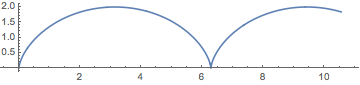
\includegraphics[scale = 0.5]{Cycloid}
\begin{equation}
  \begin{cases}
    x = r(\theta - \sin{\theta})\\
    y = r(1-\cos{\theta})
  \end{cases}
\end{equation}
$\theta$ is auxiliary variable/parameters, and $r$ is clearly the constant. Also, don't forget the range: $0 \le \theta \le 2\pi$.\footnote{Don't forget about the range of parameter!  Especially for the test.}

\paragraph{Slope, Derivatives}
For
\begin{equation}
  \begin{cases}
    x = f(t)\\
    y = g(t)
  \end{cases}
\end{equation}
Note that the tangent line is a relative notion with specific point on a curve. With parameter t, every point of curve could be described by t and t only. We have point $(x_0, y_0)$:
\begin{equation}
  \begin{cases}
    x_0 = f(t_0) \to \frac{dx}{dt} = f'(t)\\
    y_0 = g(t_0) \to \frac{dy}{dt} = g'(t)
  \end{cases}
\end{equation}
$$slope = \frac{g'(t_0)}{{f'(t_0)}}$$ at $(x_0, y_0)$. 

\paragraph{}
Using chain rule\footnote{It literally looks like $dx$ cancelled out. But no. See section 10 for clear definition of differentials}, we have: $$\frac{dy}{dt}=\frac{dy}{dx} \cdot \frac{dx}{dt}$$ $$\to \frac{dy}{dx}=\frac{ \frac{dy}{dt}}{{\frac{dx}{dt}}}$$
Through $k = \frac{g'(t_0)}{f'(t_0)}$, we learn that 1) When $g'(t_0) = 0 \text{ and } f'(t_0)\not= 0$, i.e. slope is 0, the tangent line is horizontal. 2) When $g'(t_0) \not= 0 \text{ and } f'(t_0) = 0$, the line is vertical. 3) Slope $>0$ means $y$ is increasing as $x$ is increasing. Other properties applied. 


%3
\section{Integration of Parametric Curve}
\paragraph{Area ``under the curve"}
Derived from SVC:
$$ A = \int_a^b ydx$$
We have:
$$A = \int_\alpha^\beta g(t)f'(t)dt$$
Be careful that the area could be under x axis, remember to $\int = -$Area. 
\paragraph{Arc Length}
Derived from SVC:
$$L = \int_a^b \sqrt{1+(\frac{dy}{dx})^2}dx$$
and the real essence of arc length formula is really the distance formula $z = \sqrt{x^2 + y^2}$:
$$L = \int_\alpha^\beta \sqrt{(\frac{dx}{dt})^2 + (\frac{dy}{dt})^2}dt$$

\paragraph{Area of a revolution surface}
Same reasoning:
$$S = \int_\alpha^\beta 2\pi g(t) \sqrt{(\frac{dx}{dt})^2 + (\frac{dy}{dt})^2}dt$$

%4
\section{Polar Coordinate}
Formal definition: $$r\text{: Distance between origins and the point}$$$$\theta \text{: Angle between the line connecting point and origin with positive x axis}$$ $$ P\to (r_0,\theta_0)$$
We also define polar function:
$$r = F(\theta)$$
\begin{equation}
  \begin{cases}
    x_0 = r_0 \cos(\theta_0) = F(\theta_0) \cos(\theta_0)\\
    y_0 =  r_0 \sin(\theta_0) = F(\theta_0) \sin(\theta_0)
  \end{cases}
\end{equation}
In sense, we can see polar function is parametric. In a sense, it is a "higher order function", that one function calls or define another function. 
\paragraph{}
We graph polar function through two different system, cartesian and polar: 
\paragraph{}
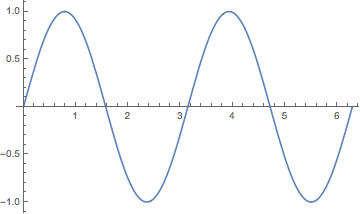
\includegraphics[scale = 0.5]{polarcar}
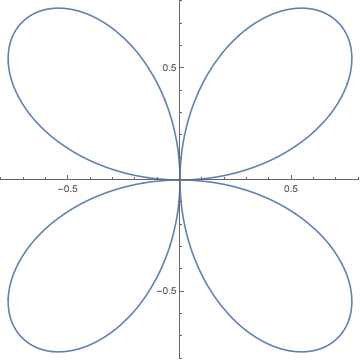
\includegraphics[scale = 0.3]{polar}
\paragraph{}
Now we have the x and y. We can get the derivative, tangent line, and arc length through formulas from section 4. However, area: $$A = \frac{1}{2} f(\theta)^2 \delta \theta$$ $$ = \int_\alpha^\beta \frac{1}{2} f(\theta)^2 de$$
One more thing, the transformation between polar and cartesian is easy: just remember few basic rules:
\begin{equation}
  \begin{cases}
    x = r \cos(\theta)\\
    y =  r\sin(\theta)\\
    x^2 + y^2 = r^2 \\
    \theta = \tan{\frac{y}{x}}
  \end{cases}
\end{equation}

%5
\section{Vectors}
\paragraph{3D Space}
In 1D, a line is drawn. Every geometric object on this line is assigned an algebraic value. \\
In 2D, a plane is drawn. Every point on the plane is imposed a coordinate. A collection of numbers as addresses of points on plane fully describe $\mathbb{R}^2$\\
In 3D, a space is drawn. We use perspective to represent or visualize the 3D space on our plane/paper.

\paragraph{Discussion on orientation and degree of freedom in different dimensions}
In 1D, there are two orientation for the line. Left to right or right to left. It cannot be rotated nor switched. 
In 2D, there are two orientation for the plane. Either x-y or y-x. These two orientations are independent and exclusive. 
In 3D, there are also only two orientations. Remember to use right hand rule. 

\paragraph{Properties}
For point $P(x_0,y_0,z_0)$ and $p(x_1,y_1,z_1)$: $$d(P,Q) = \sqrt{(x_0-x_1)^2+(y_0-y_1)^2+(z_0-z_1)^2}$$
Unfold this, we have expression of sphere in 3D: $$ (x_0-x_1)^2+(y_0-y_1)^2+(z_0-z_1)^2 = r^2 $$

\paragraph{Vectors}
How do you really define vector? Object that has magnitude and direction. Note: just same direction and magnitude, not location! Vector is not static. It is about the movement, trajectory, the process. There could be many "lines" represent the same vector. Nevertheless, there is a numeric way to represent vector in cartesian coordinate system. \\
Given $\vec{a}$, first arrange so that initial point is $O = (0,0)$ and the end point is $P(x_0,y_0)$. We could denote: $\vec{a} = <x_0, y_0>$. Note that P is the end of the process $\vec{a}$, not the movement itself. Same in $\mathbb{R}^3$

\paragraph{Dot Product}
Result is a scaler.\\
Geometric Way: 
$$\vec{a} \cdot \vec{b} = |\vec{a}| |\vec{b}| \cos \theta$$ 
$$|\vec{a}| = \sqrt{x_0^2+y_0^2+z_0^2}$$
Algebraic Way:
$$\vec{a} = <x_0, y_0, z_0>$$ 
$$\vec{b} = <x_1, y_1, z_1>$$
$$\vec{a} \cdot \vec{b} = x_0x_1+y_0y_1+z_0z_1$$

\paragraph{Cross Product}
Get a vector, direction is perpendicular to both.\\
Geometric Way:
$$|\vec{a} \times \vec{b}| = |\vec{a}| |\vec{b}| \sin \theta$$ 
Algebraic Way:
$$|\vec{a} \times \vec{b}| = \det \begin{bmatrix} \vec{i} & \vec{j} & \vec{k} \\ x_0 & y_0 & z_0 \\ x_1 & y_1 & z_1 \end{bmatrix}$$

%6
\section{Vector in 3D Space}
\paragraph{Line in 3D}
For vector $\vec{PQ}$ on the line to be expressed, and $\vec{PQ} = t\vec{v}$: 
$$\vec{r} = \vec{v_0} + t\vec{v}$$
We can parameterize it:
\begin{equation}
  \begin{cases}
    x = x_0 + ta\\
    y = y_0 + tb\\
    z=  z_0 + tc
  \end{cases}
\end{equation}
OR:
$$\frac{x-x_0}{a}=\frac{y-y_0}{b}=\frac{z-z_0}{c}$$
Note: This representation is not unique, we could choose another point $p' = <x_0', y_0', z_0'>$ instead of P and another vector $\vec{v}$ which must be proportional to $\vec{v}$.

\paragraph{Discussion on describing object and its relation to equation}
General rule: In N dimensional space, to describe S, we need (n-d) equation. \\
In 3D, n = 3: \\
\indent To describe a point ($d = 0$),  $n - d =3$. You need to impose three equations. \\
\indent For a line, $ n -d = 2$. Two equations\\
\indent For a plane, just one equation will suffice.

\paragraph{Equation of a (flat) plane}
We use the normal vector, to pinpoint a plane. We have point $P(0, 0, 0), Q(x, y, z)$ and $\vec{n} = <a,b,c>$
$$\vec{PQ} = \vec{r} - \vec{r_0}$$ $$\text{Since } \vec{PQ} \perp \vec{n} \Rightarrow \vec{PQ} \cdot \vec{n} = 0 $$ 
$$<x -x_0, y-y_0, z-z_0> \cdot <a,b,c> = 0$$
$$a(x-x_0) + b(y-y_0) + c(z-z_0) = 0$$

%7
\section{Surfaces in 3D Space}
See textbook Chapter 12.6. \\
General rule: Building upon the conics in 2D, you should be able to infer its corresponding 2D surface in 3D. 

%8
\section{Vector Function}
Curve in 3D: 
\begin{equation}
  \begin{cases}
    x = f(t)\\
    y = g(t)\\
    z=  h(t)
  \end{cases}
\end{equation}
Therefore, we have: $$\vec{r}(t)=<f(t), g(t), h(t)>$$
\paragraph{Example of spiral curve}
\begin{wrapfigure}{r}{0.25\textwidth}  %this figure will be at the right
    \centering
    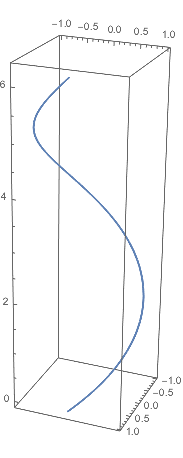
\includegraphics[scale = 0.3]{spiral}
\end{wrapfigure}
For function:\\
\begin{equation}
  \begin{cases}
    x = \cos t\\
    y = \sin t \\
    z=  t
  \end{cases}
\end{equation}
Its projection on xy plane is a circle. \\
Now we can find the direction vector $\vec(v)$ at, say, $\frac{\pi}{4}$:
$$\vec{r}(t) = \vec{r_0} + \vec{v}t$$
$$\vec{r_0} = <\cos{\frac{\pi}{4}}, \sin{\frac{\pi}{4}}, \frac{\pi}{4}> = < \frac{\sqrt{2}}{2},\frac{\sqrt{2}}{2} , \frac{\pi}{4}>$$
$$\vec{v} = \vec{r}'(t_0) = < -\frac{\sqrt{2}}{2} , \frac{\sqrt{2}}{2} , 1>$$
Therefore, the tangent lane:
$$ \vec{r}(s) = < \frac{\sqrt{2}}{2},\frac{\sqrt{2}}{2} , \frac{\pi}{4}> + < -\frac{\sqrt{2}}{2} , \frac{\sqrt{2}}{2} , 1>s$$

\paragraph{Regarding function with more than one variable}
Be careful with the domain. 
\paragraph{Finding the limit of a multivariable function} 
Rule: Approach it along various curve/equation/function, if all of them yield the same result, then the limit is the result. It not, the limit doesn't exist. Generally, you should test for two cases. 




%9
\section{Derivatives}
\paragraph{In single variable...}
$$f'(x) = \lim_{\Delta x \to 0} \frac{f(x_0 + \Delta x) - f(x_0)}{\Delta x}  \text{ if it exist.} $$
Geometrically, it is the slop of the tangent line at point $x$, and the linear approximation of the line at point $x$, the instantaneous rate of change.
\paragraph{Partial Derivatives}
As for $f(x,y)$, we take two derivatives: with respect to x and to y. 
$$f_x(x_0,y_0) = \lim_{\Delta x \to 0} \frac{f(x_0 + \Delta x, y_0) - f(x_0, y_0)}{\Delta x}  $$
$$f_y(x_0,y_0) = \lim_{\Delta y \to 0} \frac{f(x_0, y_0 + \Delta y) - f(x_0, y_0)}{\Delta y}  $$
When we are taking $f_x$, we use $y$ as a constant. Vice versa. Interestingly: 
$$f_xy = f_yx$$

\paragraph{Tangent Plane}
We can see tangent plane as the plane consist of two tangent lines. 
Or we derive from curve:
$$y - y_0 = f'(x_0)(x-x_0)$$
$$\to$$
 $$z - z_0 = f_x(x_0, y_0)(x-x_0)+f_y(x_0,y_0)(y-y_0)$$


%10
\section{Differentials, Tangent Planes and Linear Approxiamation}
\subsection{Tangent Planes}
Suppose $f$ has continuous partial derivatives. An equation of the tangent plane to the surface $z = f(x,y)$ at the point $P(x_0,y_0,z_0)$ is $$z - z_0 = f_x(x_0, y_0)(x-x_0)+f_y(x_0,y_0)(y-y_0)$$
\subsection{Linear Approximation}
The resulted tangent plane $z - z_0 = a(x-x_0)+a(y-y_0)$ is particularly helpful for computing linear approximations of two variables. From previous equation $$z - z_0 = f_x(x_0, y_0)(x-x_0)+f_y(x_0,y_0)(y-y_0)$$ We have  $$z = z_0 + f_x(x_0, y_0)(x-x_0)+f_y(x_0,y_0)(y-y_0)$$  The linear function whose graph is the tangent plane based on point $(x_0, y_0, f(x_0, y_0))$: $$z = L(x, y) = f(x_0,y_0)+f_x(x_0, y_0)(x-x_0)+f_y(x_0,y_0)(y-y_0)$$ is called linearization of $f$ at $(x_0, y_0)$. Furthermore, the approximation $$ f(x, y) \approx f(x_0,y_0)+f_x(x_0, y_0)(x-x_0)+f_y(x_0,y_0)(y-y_0)$$ is called the linear approximation or the tangent plane approximation of $f$ at $(x_0, y_0)$.
\paragraph{}
Now we continue to find the corresponding increment of z: $$\Delta z = f(a+\Delta x, b+\Delta y) - f(a,b)$$ From the increment, we can define: 
If $z = f(x, y)$, then $f$ is differentiable at $(a,b)$ if $\Delta z$ can be expressed in the form $$\Delta z = f_x(a, b)\Delta x +  f_y(a, b)\Delta y  + \varepsilon_1\Delta x+  \varepsilon_2\Delta y$$where $\varepsilon _1 and \varepsilon _2 \to 0$ as $(\Delta x, \Delta y) \to (0,0)$.

Sometimes you can't use equation above to check the differentiability of a function. Nevertheless: If the partial derivative $f_x$ and $f_y$ exist near (a,b) and are continuous at $(a,b)$, then $f$ is differentiable at (a,b)\footnote{which makes a lot of sense because if the two partial derivative (i.e. the tangent lines on x or y direction) is differentiable, the plane must be differentiable.}

\paragraph{Parameterization}
For point $p(2, 3)$ and function $f(x,y)$, 
$$f(\delta x_p, \delta y_p) = f(<2,  3>) + <{\delta f \over {\delta x}}, {\delta f \over {\delta y}}> \cdot <\delta x, \delta y>$$

\subsection{Differentials}
\subsubsection{Misconception}
In single variable calculus, we often see that, for $f(x)$: $$df = f'(x)dx$$ $$f' = dy /dx$$ Student then ask: Does $f'$ have independent meaning? Shouldn't it just be $df\over dx$? Wrong. $f'$ has independent meaning because it represent the derivative of function $f$ at point $x_0$. 
\subsubsection{Differentials in One Variable}
\paragraph{Definition} 
The differential of $f(x)$ at the point $x_0$ is the function of $x$ defined by $$f(x) - f(x_0) = f'(x_0)(x-x_0)$$ Note that the differential is attach to a particular point, just like the tangent line. The function depends on $x_0$. Now, we give $f(x) - f(x_0)$ a notation $df_{x_0}^{(x)}$. It is a function of $x$ whoes graph is the tangent line at $x_0$, up to shift by $f(x_0)$: $$ df_{x_0}^{(x)} = f'(x_0)(x-x_0)$$
Furthermore, we give $x-x_0$ a notation\footnote{Note how all three variables depend on the starting point $x_0$, here we answer the misconception question: $f'$ has independent meaning. And it depends on $x_0$}: $$ df_{x_0}^{(x)} = f'(x_0)d_{x_{x_0}}$$
\paragraph{Linear Approximation and Error Bound in One Variable}


We have 

\begin{equation} 
\begin{split}
\Delta f & =f(x_0+\Delta x) - f(x_0) \\
	& = f'(x_0)(x-x_0) + Error \\
	& = df_{x_0} + \varepsilon (x)(x-x_0) \\ 
	where \varepsilon (x)\to 0 as x \to 0
\end{split}
\end{equation}

The linear part of $\Delta f$ we call it differential. It is linear for $(x - x_0)$. \footnote{For more information, you can look at Taylor Series at $x_0$ and the error bound for each following terms. As $x \to 0$, quadratic and cubic terms get smaller in a much faster rate.} This is the idea of linear approximation. Since the linear term dominant. 
\paragraph{Back to multivariable}
For the same procedure, we now have the differential of $dz$, which we call it total differential: $$dz = f_x(x,y)dx + f_y(x,y)dy = {\delta z \over \delta x} dx +  {\delta z \over \delta y} dy$$

The operation of three and more variables should follow the same procedure. 

%14.5
\section{Chain Rule (14.5)}
From a certain standpoint, chain rule is the operation of derivative on higher order functions. In one variable, if $y=f(x)$ and $x = g(t)$, $$\frac{dy}{dt}=\frac{dy}{dx}\frac{dx}{dt}$$
Note that $dx$ does not ``cancel" out, it is more subtle than that.

In multivariable case, however, the dependency relationship becomes more complex.
\paragraph{Case 1}
Suppose that $z = f(x,y), x = g(t), y = h(t)$, all differentiable, we have\footnote{It is very similar to the definition of the differential $dz = \frac{\delta z}{\delta x}dx+\frac{\delta z}{\delta y}dy$}: $$\frac{dz}{dt}=\frac{\delta f}{\delta x}\frac{dx}{dt}+\frac{\delta f}{\delta y}\frac{dy}{dt}$$
Note the dependency relationship is still fairly simple:

\Tree [.z [ t ].x [ t ].y ]

\paragraph{Case 2}
Suppose that $z=f(x,y)$, $x=g(s,t)$, $y = h(s,t)$:
$$\frac{\delta z}{\delta s}=\frac{\delta z}{\delta x}\frac{\delta x}{\delta s}+\frac{\delta z}{\delta y}\frac{\delta y}{\delta s} $$

$$\frac{\delta z}{\delta t}=\frac{\delta z}{\delta x}\frac{\delta x}{\delta t}+\frac{\delta z}{\delta y}\frac{\delta y}{\delta t}$$
The dependency tree now becomes:

\Tree [.z [[ s ] [ t ]].x [[ s ] [ t ]].y ]

Note that, in operation, we have the collapse of the tree above into: \Tree [.z [ t ].x [ t ].y ] and \Tree [.z [ s ].x [ s ].y ]. We have seperate $\frac{\delta z}{\delta s} $ and $\frac{\delta z}{\delta t}$
\paragraph{General Case}
Indeed the dependency is key. We now have the general version of the chain rule: Suppose that $u$ is a differentiable function of the $n$ variables $x_1, x_2, \ldots, x_n$ and each $x_j$ is a differentiable function of $m$ varaibles $t_1, t_2, \ldots, t_m$. Then $u$ is a function of $t_1, t_2, \ldots, t_m$ and $$\frac{\delta u}{\delta t_i}=\frac{\delta u}{\delta x_1}\frac{\delta x_1}{\delta t_i} + \frac{\delta u}{\delta x_2}\frac{\delta x_2}{\delta t_i}  + \ldots + \frac{\delta u}{\delta x_n}\frac{\delta x_n}{\delta t_i} $$ for each $i = 1, 2, \ldots, m.$

\paragraph{Implicit Function Theorem}
Suppose an equation of the form $F(x,y)=0$ defines y implicitly as a differentiable function of x, that is, $y=f(x)$, where $F(x,f(x)) = 0$ for all in the domain of f. Using chain rule to differentiable both sides, we obtain: $$\frac{\delta F}{\delta x}\frac{dx}{dx}+\frac{\delta F}{\delta y}\frac{dy}{dx} = 0$$ Since $\frac{dx}{dx} = 1$, we obtain: $$\frac{dy}{dx} = -\frac{\frac{\delta F}{\delta x}}{\frac{\delta F}{\delta y}} = -\frac{F_x}{F_y}$$
For more variables, we apply the same logic: \par Suppose now $z = f(x,y)$. Differentiate $F(x,y,z)=0$, we have: $$\frac{\delta F}{\delta x}\frac{\delta x}{\delta x}+\frac{\delta F}{\delta y}\frac{\delta y}{\delta x} + \frac{\delta F}{\delta z}\frac{\delta z}{\delta x}= 0$$ But $\frac{\delta x}{\delta x} = 1$ and $\frac{\delta}{\delta x}(y) = 0$, we have:
$$\frac{\delta z}{\delta x} = -\frac{\frac{\delta F}{\delta x}}{\frac{\delta F}{\delta z}}$$
$$\frac{\delta z}{\delta y} = -\frac{\frac{\delta F}{\delta y}}{\frac{\delta F}{\delta z}}$$
%14.6
\section{Directional Derivatives and the Gradient Vector(14.6)}
Partial derivatives $fx$ and $fy$ represent the rates of the change of f in the $x-$ and $y-$ directions, that is, in the directions of the unit vectors $\vec{i}$ and $\vec{j}$. These two derivatives are fairly limited, therefore, we define the \emph{directional derivative} of $f$ at $(x_0,y_0)$ in the direction of a unit vector $\vec{u} = <a,b>$: $$D_uf(x_0,y_0) = \lim_{h\to0}\frac{f(x_0+ha, y_0+hb)-f(x_0,y_0)}{h}$$ Note that, for now, the partial derivatives of $f$ with respect to $x$ and $y$ are just special cases of the directional derivative since we can just let $\vec{u} = \vec{i} \text{ or } \vec{j}$.

\par
With any \textbf{unit vector} $\vec{u} = <a,b>$. We also have: $$D_uf(x,y)=f_x(x,y)a + f_y(x,y)b$$
$D_uf(x,y)$ can be expressed as dot product of two vectors: $$D_uf(x,y) = <f_x(x,y),f_y(x,y)>\cdot \vec{u}$$
We denote that the \emph{gradient} of $f$ is the vector function $\nabla f$: $$\nabla f(x,y) = <f_x(x,y),f_y(x,y)> = \frac{\delta f}{\delta x} \vec{i} + \frac{\delta f}{\delta y}\vec{j}$$
Finally: $$D_uf(x,y)=\nabla f(x,y)\cdot\vec{u}$$

\par
Same rules apply for three or more variables.
\paragraph{Maximizing the Directional Derivative}
Since $\vec{u}$ is a unit vector: $$D_uf = \nabla f \cdot \vec{u} = |\nabla f| \cos{\theta}$$
When $\nabla f$ is in the same direction as $\vec{u}$, i.e. $\theta = 0$, $D_uf$ is maximized. Reverse direction, minimized. Perpendicular, zero.

\paragraph{Tangent Planes to Level Surfaces}
For a point $P(x_0,y_0,z_0)$ on level surface $F(x,y,z) = k$, and for curve on the surface can be represented by $\vec{r}(t) = <x(t), y(t), z(t)>$, we have:
$$F(x(t),y(t),z(t))=k$$
$$\frac{\delta F}{\delta x}\frac{\delta x}{\delta t} + \frac{\delta F}{\delta y}\frac{\delta y}{\delta t}+\frac{\delta F}{\delta z}\frac{\delta z}{\delta t} =0$$
Since  $\nabla F = <F_x, F_y, F_z>$ and $\vec{r}'(t) = <x'(t),y'(t),z'(t)>$: $$\nabla F\cdot \vec{r}'(t) = 0$$
$\nabla F$ is the normal vector to the tangent plane. Plug in $t = t_0$ and $<x_0, y_0, z_0>$, we have the equation for the tangent plane to the level surface at point $P$: $$F_x(x_0,y_0,z_0)(x-x_0)+F_y(x_0,y_0,z_0)(y-y_0)+F_z(x_0,y_0,z_0)(z-z_0) = 0$$ And the equation of the \emph{normal line} is: $$\frac{x-x_0}{F_x(x_0,y_0,z_0)} = \frac{y-y_0}{F_y(x_0,y_0,z_0)} = \frac{z-z_0}{F_z(x_0,y_0,z_0)}$$



%14.7
\section{Extremas (14.7)}
\paragraph{Definition} A function of two variables has a local maximum at $(a,b)$ if $f(x,y)\leq f(a,b)$ when $(x,y)$ is near $(a,b)$. The number $f(a,b)$ is called a local maximum value. If $f(x,y)\geq f(a,b)$ when $(x,y)$ is near $(a,b)$. The number $f(a,b)$ is called a local minimum value.
\paragraph{Theorem} If $f$ has a local maximum or minimum at $(a,b)$ and the first-rder partial derivatives of $f$ exist there, then $f_x(a,b) = 0$ and $f_y(a,b)=0$.
\paragraph{Second Derivative Test} Suppose the second partial derivatives of $f$ are continuous on a disk with center $(a,b)$, and suppose that $f_x(a,b)=0$ and $f_y(a,b) = 0$ [that is, $(a,b)$ is a critical point of $f$]. Let $$ D = D(a,b) = f_{xx}(a,b)f_{yy}(a,b) -[f_{xy}(a,b)]^2$$
If $D > 0$ and $f_{xx}(a,b) > 0$, then $f(a,b)$ is a local minimum.
\par
If $D > 0$ and $ f_{xx}(a,b) < 0$, then $f(a,b$) is a local maximum.
\par
If $D < 0$, then $f(a,b)$ is not a local maximum or minimum. The point $(a,b)$ is called a saddle point of $f$ and the graph of $f$ crosses its tangent plane at $(a,b)$.
\par
If $D = 0$, the test gives no information.
\par
It is helpful to write $D$ as determinant of matrix $D = det \begin{bmatrix} f_{xx} & f_{xy}  \\ f_{yx} & f_{yy} \end{bmatrix}$
\paragraph{Extreme Value Theorem for Functions of Two Variables} If $f$ is continuous on a closed, bounded set $D$ in $\mathbb{R}^2$, then $f$ attains an absolute maximum value $f(x_1,y_1)$ and an absolute minimum value $f(x_2,y_2)$ at some points $(x_1,y_1)$ and $(x_2,y_2)$ in $D$.
\par
A closed set in $\mathbb{R}^2$ is one that contains all its boundary points. A bounded set in $\mathbb{R}^2$ is one that is contained within some disk. It is finite in extent.


%14.8
\section{LaGrange Multiplier (14.8)}
For maximizing or minimizing a general function $f(x,y,z)$ subject to a constraint (or side condition) of the form $g(x,y,z) = k $. The result happens where the objects touch each other $\to$ common tangent line $\to$ identital normal lines $\to$ parallel gradient vector at point.
\par
\emph{The method of Lagrange Multipliers   } To find the maximum and minimum values of $f(x,y,z)$ subject to the constraint $g(x,y,z) = k$: 1) Find all values of $x,y,z,\lambda$ such that $$\nabla f(x,y,z) = \lambda \nabla g(x,y,z) $$ and $$g(x,y,z) = k$$ 2) Evaluate $f$ at all the points $(x,y,z)$ that result from step (1). The largest of these values is the max value of $f$; the smallest is the min.
\par
For a function subject to two constraint, we have: $$\nabla f(x_0, y_0, z_0) = \lambda \nabla g(x_0, y_0, z_0) + \mu \nabla h(x_0, y_0, z_0)$$
\par
Note: pay attention to the ``domain" of the constraint. The constraint need to be closed and bounded. Otherwise, there might not be both max and min from LaGrange multiplier operation. E.g. $xy=1$ in $f(x,y)=x^2 + y^2$only admits a minimum but no max.


%15.1 & 15.2
\section{Double Integrals (15.1 \& 15.2)}
Now we are exiting differential calculus and entering into the field of integral calculus. These two sides of calculus are much more subtle than just being the ``opposite".

In single variable calculus, we have a function $f(x)$, in the interval of $[a,b]$, we call $\int_{a}^{b}f(x)dx$ its integral. We now explore:

\begin{itemize}
\item \emph{Definition} For function $y = f(x)$ with interval $[a,b]$, we divide x into small interval of $\Delta x = \frac{b-a}{n}$. We take the sum of total areas of the ``rectangles'' created by the intervals. $$\sum_{i=1}^{n} f(x_i^\ast)\Delta x, x_i^\ast = \frac{x_{i+1}+x_i}{2}$$ $$\text{as }n \to \infty$$ $$\text{Area } = \int_{a}^{b}f(x)dx$$
\item \emph{Interpretation} It is the area ``under the graph''.
\item \emph{Calculation Tools} Fundamental Theorem of Calculus (in single variable): $$\int_a^b f(x)dx = F(b) - F(a), F'(x) = f(x)$$
\end{itemize}

Carry over to Multivariable:
\begin{itemize}
\item \emph{Definition} Limit of ``Double Riemann Sum" or as Prof. Frenkel calls it the ``Skyscraper" $$\sum_{i=1}^N \sum_{i=1}^{M} f(x_i^\ast, y_i^\ast) \Delta x \Delta y$$ $$\text{as } N,M \to \infty$$ $$\int \int f(x,y) dA$$
\item \emph{Interpretation} It is then the volume ``under the graph".
\item \emph{Calculation Tools} First evaluate one inside, then another. It is simply evaluation of integrated integral. Do it with respect to one variable, then to another.
\end{itemize}

\paragraph{Fubini theorem} the two iterated integrals $\int_a^b \int_c^d \dots dxdy$ and $\int_c^d \int_a^b \dots dydx$ are the same as long as $f(x,y)$ is continuous over the domain. Geometrically, it is simply evaluating the volume in different ways.
\paragraph{Average Value} $$f_{ave} = \frac{1}{A(R)}\iint f(x,y)dA$$
\paragraph{Type I regions}
If f is continuous on a type I region $D$ such that $$D = \{(x,y)|a\le x\le b, g_1(x)\le y \le g_2(x)\}$$ then $$ \iint \limits_D f(x,y) dA = \int_a^b \int_{g_1(x)}^{g_2(x)} f(x,y) dy dx$$
\paragraph{Type II regions}
If f is continuous on a type II region $D$ such that $$D = \{(x,y)|c\le y\le d, h_1(y)\le x \le h_2(y)\}$$ then $$ \iint \limits_D f(x,y) dA = \int_c^d \int_{h_1(y)}^{h_2(y)} f(x,y) dx dy$$
\paragraph{Note}
During integration, sometimes it is beneficial to change the order of $dx \& dy$. Just be careful that during such transformation, be attentative to Type I and Type II transformation.

%15.3
\section{Double Integrals in Polar Coordinates (15.3)}
\paragraph{Derivation of the Formula}
In general, double intergrals is about the volume. In $\int_c^d\int_a^b f(x,y)dxdy$, we are trying to find the volume fo solid ``under the graph".
Previous method is Double Riemann Sum, taking $\sum_{i=1}^N\sum_{j=1}^M f(x_i^\ast, y_i^\ast)\Delta x \Delta y$, in which $\Delta x \Delta y$ is the area of the base, while $f(x,y)$ being the height.
\par
In polar, we break our region not into cartesian rectangle but in ``poalr rectangles".
$$x_i \leq x \leq x_i + \Delta x = x_{i+1}$$
$$y_j \leq y \leq y_j + \Delta y = y_{j+1}$$
$$\to$$
$$r_i \leq r \leq r_i + \Delta r = r_{i+1}$$
$$\theta_j \leq \theta \leq \theta_j + \Delta \theta = \theta_{j+1}$$
$$\text{then}$$
$$\text{area } \neq \Delta r \Delta \theta$$
$$\text{area } = \text{``the arc" } * \Delta r = (\Delta \theta r_i)\Delta r$$
In addition to property $$r^2 = x^2 + y^2, x = r\cos(\theta), y = r\sin(\theta)$$
So we have the formula, $0\leq a \leq r \leq b$, $\alpha \leq \theta \beta$, where $0 \leq \beta - \alpha \leq 2\pi$:
$$\iint \limits_R f(x,y) dA = \int_\alpha^\beta \int_a^b f(r \cos(\theta),r\sin(\theta))r dr d\theta$$
\paragraph{Type I} also applies, i.e.
$$\iint \limits_D f(x,y) dA = \int_\alpha^\beta \int_{h_1(\theta)}^{h_2(\theta)} f(r\cos(theta), r\sin(theta))rdrd\theta$$


%15.4, 15.6
\section{Applications of Double Integrals (15.4) and Triple Integrals (15.6)}
Various Applications of Double Integrals includes:
\begin{itemize}
\item{\emph{Volume}}
\item{\emph{Density and Mass}: $$m = \lim_{k,l\to\infty}\sum_{i=1}^k\sum_{j=1}^l\rho(x_{ij}^\ast, y_{ij}^\ast)\Delta A = \iint \limits_D \rho(x,y)dA$$
}
\item{\emph{Moments and Centers of Mass:} Moment is defined as $mr$.
$$\bar{x} = \frac{M_y}{m} = \frac{\iint \limits_D x\rho (x,y)dA}{\iint \limits_D \rho (x,y)dA}$$
}
\item{\emph{Moment of Inertia:} $mr^2$
$$I_x = \iint \limits_D y^2 \rho(x,y) dA$$
Polar moment of inertia / moment of inertia about the origin, $I_0 = I_x + I_y$: $$I_0 = \iint \limits_D (x^2 + y^2)\rho(x,y) dA$$
}
\item{\emph{Probability:} Probabiltiy Density Function, the probability that $X$ lies between $a$ and $b$ and $Y$ lies between $c$ and $d$: $$P(a \leq X \leq b, c \leq Y \leq d) = \int_a^b \int_c^d f(x,y) dy dx$$
If $X$ and $Y$ are independent random variables: $$f(x,y)=f_1(x)f_2(y)$$
\par
If $f$ is a probability density fnction, then $f(x)\leq0$ and $\int_{-\infty}^{\infty}f(x)dx$
}
\item{\emph{Expected Values:}
For random variable $X$ with probability density function $f$, its mean is: $$\mu = \int_{-\infty}^\infty xf(x)dx$$
$X-mean$ and $Y-mean$ is then: $$\mu_1 = \iint \limits_{\mathbb{R}^2} xf(x, y)dA$$
$$\mu_2 = \iint \limits_{\mathbb{R}^2} yf(x, y)dA$$

}
\end{itemize}
\paragraph{Triple Integral}
The expansion of domain into another dimension gives more intesting cases. However, the genral method remains unchanged: project the function into one plane, and restrict other varaible based on that.
\paragraph{Definition and Fubini's Theorem} Rectangular box $B = [a,b] * [c, d] * [r,s]$:
$$\iiint \limits B f(x,y,z)dV = \lim_{i,m,n\to\infty} \sum_{i=1}^l\sum_{j=1}^m\sum_{k=1}^n f(x_{ijk}^\ast, y_{ijk}^\ast,z_{ijk}^\ast)\Delta V = \int_r^s \int_c^d \int_a^b f(x,y,z) dxdydz$$
\paragraph{Evaluation and Computational Tool}:
$$\iiint \limits_E f(x,y,z)dV = \int_a^b \int_{g1(x)}^{g2(x)} \int_{u1(x,y)}^{u2(x,y)} f(x,y,z)dzdydx$$
\paragraph{Application:} Instead of hypervolume in four-dimensions, triple integral is extremely useful for evaluation of 3D volume ($V(E) = \iiint \limits_E dV$), mass, moements, center of mass, moment of inertia, electric charge, joint density function, and more \dots

%15.7 & 15.8
\section{Cylindrical (15.7) and Spherical (15.8) Coordinates}
In the cylindrical coordinate system, a point $P$ is represented by $(r, \theta, z)$, where $r$ and $theta$ are polar coordinates of the porjection of $P$ onto the $xy$-plane and $z$ is the directional distance from $xy$ plane to $P$. Therefore: $$x=r\cos{\theta},y=r\sin{\theta},z=z$$ $$r^2 = x^2 +y^2, \tan{\theta}=\frac{y}{x}, z=z$$ $$\iiint \limits_E f(x,y,z)dV = \int_{\alpha}^{\beta}d\theta \int_{h_1(\theta)}^{h_2(\theta)} dr \int_{u_1(r\cos{\theta}, r\sin{\theta})}^{u_2(r\cos{\theta}, r\sin{\theta})} f(u_1(r\cos{\theta}, r\sin{\theta}), z)r dz$$
Don't forget the $r$!

%15.9 From Apostol and Stewart
\section{Change of variables (15.9)}
Variable changes in one dimension is farmiliar: $$\int_a^b f(x)dx = \int_c^d f[g(t)]g'(t)dt$$
How do we transform two dimensional $\iint_S f(x,y)dxdy$ to $\iint_T F(u,v)dudv$? We have \emph{change of variable in a double integral.} 
For sure we have following parametrization:
$$x = X(u,v), y = Y(u,v)$$
Geometrically, the two equation can be thought of mapping one region to another. The region of $x,y$ can be therefore defined or mapped by vector equation $$\vec{r}(u,v) = X(u,v)\vec{i} + Y(u,v)\vec{j}$$
The formula of transformation is $$\iint_S f(x,y)dxdy = \iint_T f[X(u,v), Y(u,v)]|J(u,v)|dudv.$$The factor $J(u,v)$ replaces $g'(t)$ in our one-dimensional formula. This factor is called the $Jocabian$ of the mapping defined by $x = X(u,v), y = Y(u,v)$. It is equal to the determinant $$J(u,v) = \det{\begin{vmatrix}
   \frac{\delta X}{\delta u} & \frac{\delta Y}{\delta u} \\
   \frac{\delta X}{\delta v} & \frac{\delta Y}{\delta v}
\end{vmatrix}
}$$
How do we get this? The transformation of a rectangle in $u,v$ region to a surface in $x,y$ can be interpreted as magnitude of cross product that describe the edge: 
$$\vec{V_1} = \frac{\delta \vec{r}}{\delta u} = \frac{\delta X}{\delta u}\vec{i} + \frac{\delta Y}{\delta u}\vec{j}$$
$$\vec{V_2} = \frac{\delta \vec{r}}{\delta v} = \frac{\delta X}{\delta v}\vec{i} + \frac{\delta Y}{\delta v}\vec{j}$$
$$\Delta u \Delta v \to |(\vec{V_1} \Delta u) \times (\vec{V_2} \Delta v)|$$
$$= |\vec{V_1} \times \vec{V_2} | \Delta u \Delta v$$
$$\vec{V_1} \times \vec{V_2} = \begin{vmatrix}
  \vec{i}&  \vec{j}& \vec{k} \\
  \frac{\delta X}{\delta u} & \frac{\delta Y}{\delta u}& 0\\
  \frac{\delta X}{\delta v} & \frac{\delta Y}{\delta v} &0
\end{vmatrix}
= \begin{vmatrix}
   \frac{\delta X}{\delta u} & \frac{\delta Y}{\delta u} \\
   \frac{\delta X}{\delta v} & \frac{\delta Y}{\delta v}
\end{vmatrix} \vec{k}
= J(u,v)\vec{k}
$$


%16.1
\section{Vector Field}
In Vector Calculus, we combined everything we had learned so far: differential calculus and intergation calculus. We are going to deduce a multi-dimensional analogues to Fundamental Theorem of Single Variable Calculus and re-define integration and differential through such theorem.
\paragraph{Definition} Let $D$ be a set in $\mathbb{R}^2$ (a plane region). A vector field on $\mathbb{R}^2$ is a function $\vec{F}$ that assign to each point $(x,y)$ in two-dimensional vector $\vec{F}(x,y)$
Therefore: $$\vec{F}(x,y)=P(x,y)\vec{i} +Q(x,y)\vec{j}=<P(x,y),Q(x,y)>$$
Three-dimensions follows.
\paragraph{Gradient Fields}
From the definition of gradient, we have: $$\nabla f(x,y) = f_x(x,y)\vec{i}+f_y(x,y)\vec{j}$$ If there exists a function $f$ such that $\vec{F}=\nabla f$We call the vector field $F$ a conservative vector field.
And we call $f$ a potential function of $\vec{F}$.
%16.2, 16.3
\section{Line Integrals}
So far, we can only apply integral on a curve in single varialble, surface in two vars, and volume on three vars. We are always integrating $D\in \mathbb{R}^n$ for $D=n$. We have tons of unexpect possibilities await.
For example, integrating a curve in $\mathbb{R}^2$.
For the line integral of $f$ along smooth curve $C$: $$\int_C f(x,y)ds = \lim_{n\to\infty}\sum_{i=1}^n f(x_i^\ast,y_i^\ast)\Delta s_i$$
There are two meaningful approaches: (1). Arc Length (2). Vector Calculus.
Arc Length: $$\int_C f(x,y)ds = \int_a^b f(x(t),y(t))\sqrt{(\frac{dx}{dt})^2+(\frac{dy}{dt})^2}dt$$
Why don't we simply take $dx$ and $dy$? $$\int_C f(x,y)dx=\int_a^b f(x(t),y(t)) x'(t) dt$$ $$\int_C f(x,y)dy=\int_a^b f(x(t),y(t)) y'(t) dt$$
Simply: $$\int_C (Pdx+Qdy) = \int_C \vec{F}d\vec{r}$$
\paragraph{Definition} Let $\vec{F}$ be a continuous vector field defined on a smooth curve $C$ given by a vector function $\vec{r}(t)$, $a\leq t\leq b$. Then the line integral of $F$ along $C$ is
$$\int_C \vec{F}d\vec{r} = \int_a^b\vec{F}(\vec{r}(t))\vec{r}'(t)dt=\int_C \vec{F}\cdot\vec{T}ds$$
\paragraph{Fundamental Theorem for Line Integrals}
Let $C$ be a smooth curve given by vector function $\vec{r}(t)$, $a\leq t \leq b$. let $f$ be a differentiable function of two or three variables whose gradient vector $\nabla f$ is continuous on $C$. Then
$$\int_C \nabla f \cdot d\vec{r}=f(\vec{r}(b))-f(\vec{r}(a))$$
Proof:
\begin{align*}
\int_C\vec{F}d\vec{r} & = \int_a^b\vec{F}(\vec{r}(t))\vec{r}(t)dt \\
& = \int_a^b (\frac{\delta f}{\delta x}\frac{dx}{dt}+\frac{\delta f}{\delta y}\frac{dy}{dt}+\frac{\delta f}{\delta z}\frac{dz}{dt})dt \\
& = \int_a^b \frac{d}{dt} f(\vec{r}(t)) dt \\
& = f(\vec{r}(b))-f(\vec{r}(a))
\end{align*}
\par
We observe that line integrals of conservative vector fields are independent of path.
\par
$\int_C\vec{F}d\vec{r}$ is independent of path in $D$ $\iff$ $\int_C\vec{F}d\vec{r} =0$ for every closed path $C$ in $D$.
\par
For conservative vector field $\vec{F}(x,y) = P(x,y)\vec{i} +Q(x,y)\vec{j}$ is a conservative vector field, where $P$ and $D$ have continuous first-order partial derivative on a domain $D$, then throughout $D$ we have
$$\frac{\delta P}{\delta y} = \frac{\delta Q}{\delta x}$$ Converse is True only for simply-connected region. 


%16.4, Frenkel's Lecture, along with Material from Stewart, Apostol, and Munkres. 
\section{Green's Theorem}
\paragraph{Preface}
Integral contains two parts, the integrand and the region (Algebraic and geometric). To find the formula, we has the following generalization: $$\iint_{\text{ some region D } \in \mathbb{R}^2} ? dA = \int_{\text{boundary of D} \in \mathbb{R}^1} (Pdx + Qdy)$$
In the geometric lelvel, domain of integration: D $\to$ $b(D)$. In the algebraic level, ? $\leftarrow$ An orbitrary vector field $Pdx + Qdy$. We can infer that ? should be expressed in terms of $\delta$ of P and Q. ? should be equal to 0 if $<P,Q>$ is a conservative vector field for that $\int_{\text{closed curve C}} (Pdx + Qdy) = 0$
\paragraph{Green's Theorem}
$$\iint_D (Q_x - P_y)dA = \int_{b(D)} (Pdx + Qdy)$$
\paragraph{Proof}
Note that there are multiple approaches. Here's Prof. Frenkel's Approach: 
\par
From $\int_C (f_x dx + f_y dy) = \int_C \nabla f \cdot d\vec{r} = f(B) - f(A)$, we infer the general formula: 
$$\int_D dw = \int_{b(D)} w$$
We have: $w = Pdx + Qdy$,
$$dw = d(Pdx) + d(Qdy) = (dP)dx + (dQ)dy$$
$$= Pxdxdx + Pydydx + Qxdxdy + Qydydy$$
Both $dxdx$ and $dydy$ are not meaningful, $dydx = -dxdy$.
$$dw = (Q_x - P_y)dA$$
\paragraph{Area}
Green's Theorem gives the following formulas for the area of region D: $$A = \oint_C xdy = -\oint_c ydx = \frac{1}{2} \oint_C xdy-ydx$$

%16.6, 16.7
\pagebreak
\section{Parametric Surfaces and Surface Integrals}

%16.5, 16.8

\section{Curl, Stokes' Theorem}
%16.5, 16.9

\section{Divergence, Divergence Theorem}
I didn't have time to write 16.5 to 16.8. Maybe someday I will come back to it!
Sorry about that. \\
See next page for some generalization of these theorems. \\
If you have time, you can fix this! The tex file can be find here:\\
\url{https://github.com/simon-mo/PKB/tree/master/assets}

%De Rham Integral
\pagebreak
\section{An Overview of Chapter 16}
The detail of this section is adopted from Prof. Frenkel\'s note. 
\par
\emph{The purpose is outline a general formalism which allows for an uniform treatment of various integrals studied in Chapter 16}
\par
\subsection{What do we integrate?}
Start with conclusion:\emph{We are integrating m-forms.}
Which is, the differential form of degree m. 
\par
Let $Y$ be an $m$ dimensional domain in $\mathbb{R}^n (m\leq n)$. We should integrate over $$f(x_1, \ldots, x_n)dx_{i_1}dx_{i_2}\ldots dx_{i_m}$$. To integrate, we first parametrize the domain: identify it with a flat domain $Z\subset \mathbb{R}^m$ with coordinate $z_1, \ldots, z_m$. This means writing each $x_i$ as a funtion $x_i(z_1,\ldots,z_m)$. We have:
$$\int_f(x_1, \ldots, x_n)dx_{i_1}dx_{i_2}\ldots dx_{i_m} = \int_Z f\frac{\delta(dx_{i_1},dx_{i_2},\ldots ,dx_{i_m})}{\delta(z_1, z_2, \ldots, z_m}dz_1 dz_2\ldots dz_m$$

\paragraph{Example of a curve}
For a curve in 3D space: $m = 1, n = 3$, we need to integrate $Pdx + Qdy + Rdz$. To do so, we parametrize $P,Q,R$ which are function in $(x,y,z)$ into one dimensional parameter equation: $x=x(t), y=y(t),z=z(t), a\leq t \leq b$. Then we write: $$\int_C (Pdx+Qdy+Rdz) = \int_{[a,b]} (P\frac{\delta x}{\delta t} dt + Q\frac{\delta y}{\delta t} dt + R\frac{\delta z}{\delta t} dt)$$
\par
\emph{Note:} the Stewart book call it the line integral of the vector field $\vec{F} = <P,Q,R>$ over curve $C$, but Frenkel believes it is more natural to think that we are really jsut integrating $Pdx+Qdy+Rdz$.

\paragraph{Example of a surface}
For a surface in 3D space: $m = 2, n = 3$, we need to integrate $Adydz + Bdzdx + Cdxdy$. To do so, we parametrize $A,B,C$ which are function in $(x,y,z)$ into two dimensional parameter equation: $x = x(u,v), y=y(u,v),z=z(u,v), (u,v)\in D \subset \mathbb{R}^2$. Then we have change of variable $$dxdy = \frac{\delta(x,y)}{\delta(u,v)} dudv$$ where $\frac{\delta(x,y)}{\delta(u,v)} $denotes \emph{Jacobian}. Thus we flatten a surface $S$ into a \emph{flat} domain $D$ in $\mathbb{R}^2$. We can write: 
$$ \iint_S (Adydz + Bdzdx + Cdxdy) = \iint_D (A\frac{\delta(y,z)}{\delta(u,v)}+B\frac{\delta(z,x)}{\delta(u,v)}+C\frac{\delta(x,y)}{\delta(u,v)})$$

\paragraph{Case of $m=n=3$}
Interestingly, the domain is already flat. We simply treat it as an iterated integral. 

\paragraph{Recap of m-form}
In essence, $m-form$ is just $fdx_{i_1}dx_{i_2}\ldots dx_{i_m}$. 0-form is just a function. 1-form is $Pdx + Qdy + Rdz$ and 2-form is $Adydz + Bdzdx + Cdxdy$. We use parametrization shown above to integrate m-form.

\subsection{De Rham Integral}
Now we introduce operation $d$ that maufactures an $(m+1)$-form, denoted by $d\omega$, out of any $m$-form$\omega$. Therefore, we have $$d(f(x_1, \ldots, x_n)dx_{i_1}dx_{i_2}\ldots dx_{i_m}) = \sum_{j=1}^n \frac{\delta f}{\delta x_j} dx_j dx_{i_1},dx_{i_2},\ldots ,dx_{i_m}$$ as a general operation of $m$-form. The operation $d$ mapped operation to each terms. This operation if called \emph{de Rham differential}. 
\paragraph{Examples}
$\omega =  $ 0-form: $$df = \sum_{j=1}^{n} \frac{\delta f}{\delta x_j} dx_j$$
How about $\omega$ = 1-from in $\mathbb{R}^3$: $$dw = \frac{\delta P}{\delta x} dxdx + \frac{\delta P}{\delta y} dydx + \ldots$$
$$d\omega = (\frac{\delta R}{\delta y} - \frac{\delta Q}{\delta z})dydz + (\frac{\delta P}{\delta z} - \frac{\delta R}{\delta x})dzdx + (\frac{\delta Q}{\delta x} - \frac{\delta P}{\delta y})dxdy $$
The functions here are the components of curl of the vector field $<P, Q, R>$. 
\par
Let $\omega$ be a 2-form given by $Adydz + Bdzdx + Cdxdy$, going through the same procedure, we have: $$d\omega = (\frac{\delta A}{\delta x} + \frac{\delta B}{\delta y} + \frac{\delta C}{\delta z})dxdydz$$
The function on the right hind side is teh divergence of the vector field $<A,B,C>$


\end{document}  